\documentclass{article}
\usepackage[utf8]{inputenc}

\title{Informe sobre laboratorio 4: STP y creación de VLAN}
\author{Matías Castro - Patricio Inostroza}
\date{Abril 2017}

\usepackage{natbib}
\usepackage{graphicx}

\begin{document}


\begin{titlepage}

\maketitle
\huge


\end{titlepage}

\tableofcontents 
\cleardoublepage

\section{Introducción}
En el siguiente informe analizaremos el funcionamiento del protocolo STP y su influencia en la creación de una red a la hora del comienzo del tráfico de información, cómo este protocolo ayuda a evitar errores masivos dentro de una topología, además, implementaremos distintas VLAN y comprobaremos su funcionamiento, beneficios y distintos modos de usarla, todo visto a través de Packet Tracer, que nos permite simular estas redes. Finalmente resolveremos dudas que pueden darse dado esto.

\newpage

\section{Desarrollo}
\subsection{STP}
STP: Este es un protocolo que se encarga de determinar cual es la mejor ruta que debe seguir un paquete entre switchs para evitar que se genere un bucle entre enlaces que pueden ser redundantes, como podemos ver, en la Figura 1, el STP está activado, por lo que solo algunos canales están activos y los otros no, asi no se genera este problema.


\begin{figure}[h]
\centering
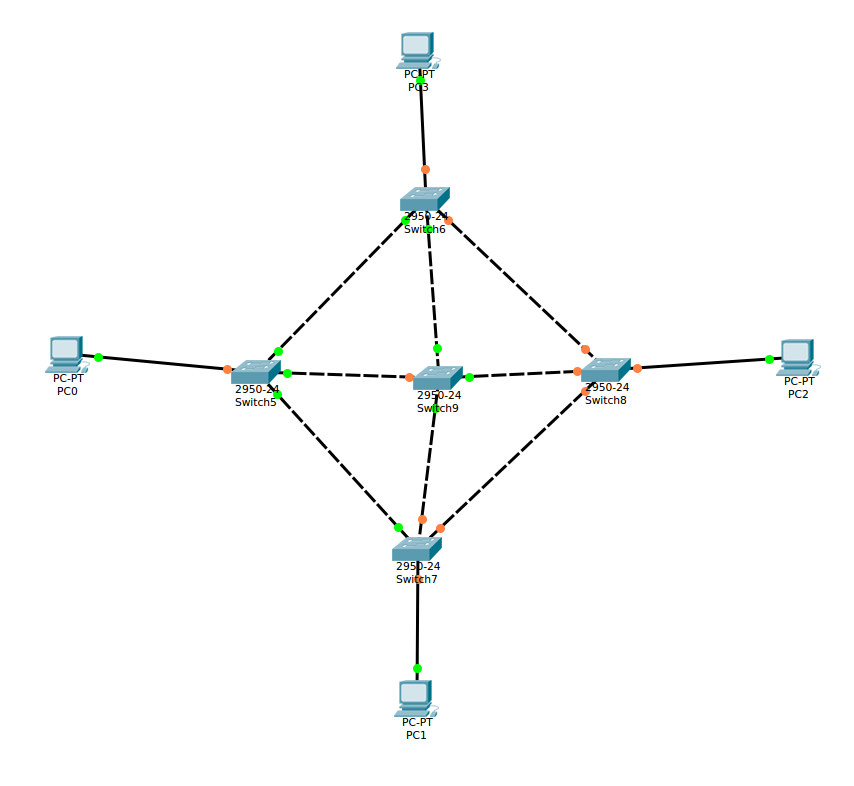
\includegraphics[scale=0.4]{STPa}
\caption{STP Activado}
\end{figure}


En la siguiente imagen (Figure 2) desactivamos el STP en todos los switchs, así todos los canales están activados (todos en verde)
\newpage

\begin{figure}[h!]
\centering
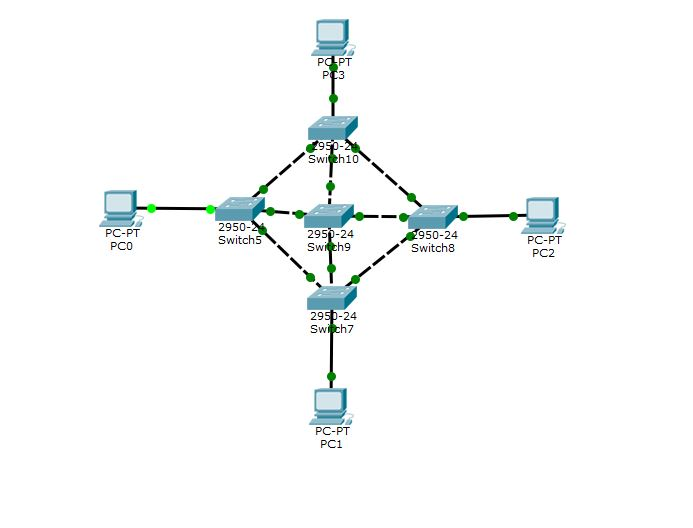
\includegraphics[scale=0.7]{STPd}
\caption{STP Desactivado}
\end{figure}

\subsection{VLAN}

Paralelo al STP, existen las VLAN, son pequeñas redes que logran separar entornos broadcast con solo unos comandos, usando switchs y no routers, por lo que podemos abaratar costos.\\
Cada VLAN posee un dominio broadcast distinto, por lo que es muy util en un entorno en el que hayan distintos grupos de trabajo que compartan la red aumentando su privacidad al separarlos.

\begin{figure}[h!]
\centering
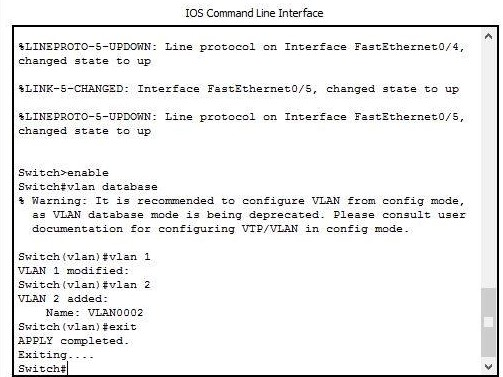
\includegraphics[scale=0.8]{vlan}
\caption{VLAN CLI}
\end{figure}

En la próxima imagen (figure 3) se observa la linea de comandos (CLI) para agregar una red VLAN a un switch.\\

\newpage

Las VLAN pueden asignar distintos protocolos a cada puerto, para saber como trabajar con el equipo al que está conectado, Nostros abordaremos dos: los puertos Trunk y los puertos Access.\\

Puertos Trunk: los puertos Trunk se usan en la comunicación de dos switchs, ya que permiten el traspaso de información sin etiquetar, así podremos usar mas de una VLAN en un switch. Su configuración en línea de comandos se puede observar en la figura 4.


\begin{figure}[h!]
\centering
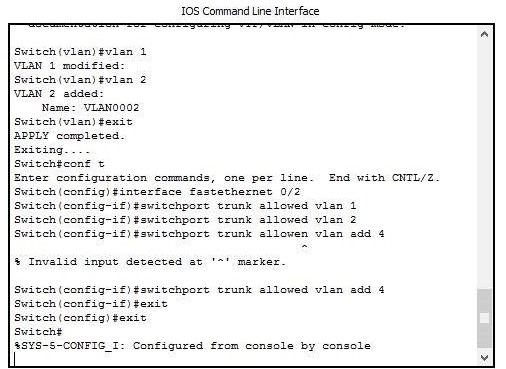
\includegraphics[scale=0.8]{trunk}
\caption{Trunk CLI}
\end{figure}


Puerto Access: Se encarga de darle al terminal(es) acceso a solo una VLAN, evitando la mezcla de dos VLAN sobretodo en switchs de 2 o mas VLAN, su configuración en CLI se observa en la figura 5.




\begin{figure}[h!]
\centering
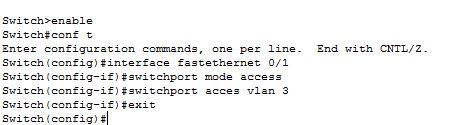
\includegraphics[scale=0.8]{access}
\caption{Access CLI}
\end{figure}

\cleardoublepage

\section{Preguntas}

1.	¿Cuál es la diferencia entre modo Trunk y modo Access? 
R:  Generalmente y como apreciamos en este informe el modo Access es para conectar dispositivos finales, así puede pasar una vlan gracias a este. Por otra parte, el modo Trunk permite el tráfico de más de una Vlan, aquí lo vimos claramente cuando conectamos un switch a otro. (Capa8,2014)

2.	¿Qué ocurre si conecto una puerta en modo Trunk a un PC? 
R:  En teoría es posible, pero es inservible dado que no se necesitan el paso de mas vlan, aparte de las que requiere y ya están agregadas para los PC de ese terminal.

3.	¿Qué ruta sigue un ping del PC 3 al PC 8? ¿Es una ruta eficiente en cuanto a tiempo? ¿Qué opción daría usted para poder llegar a los tres PC con VLAN 3 sin generar bucles y ser óptimo en tiempo? 
R: Desde el PC 3 va hacia el switch 2, después hacia el 4, después el switch 3 que es el que conecta con el PC 8. Es un ruta eficiente, ya que la otra alternativa tiene la misma cantidad de switch para llegar. Para la siguiente pregunta la otra ruta que podría haber seguido el ping es una opción optima en tiempo, en cuanto a bucles, se tendría por STP que bloquear al switch 4 para evitarlos, dado que para este desde el PC 3 al 2 es muy largo en cuanto a tiempo, y asi evitar un bucle.

4.	¿Qué pasa si conecto dos switchs uno con la puerta Trunk y la otra con puerta Access? 
R: Esto se da en la última topología de este informe, y fue por donde pudo pasar el ping desde el PC 3 al 8, uno iba por un servidor Trunk, y el otro por uno en Access, fue por este último dado que en Trunk se canaliza todo el trafico.

5.	¿Cuáles son las ventajas de este sistema llamado VLAN? Mencione al menos 3.
R: Tiene un mejor rendimiento, dado el factor de división de las redes, también con esto se reduce el número de dispositivos que pueden hacer que se produzca un envío masivo de paquetes broadcast (envíos masivos), a lo que se le llama tormenta de broadcast, esto se evita gracias a la segmentación. Y otra de las más importantes es la seguridad que genera separando a la red. (Vlan,2016)

\newpage

\section{Conclusión}
Si bien en este informe se a bordo de manera básica el funcionamiento de STP y VLAN, quedó claro lo más importante de cada uno. El primero nos permite evitar bucles en enlaces redundantes al transmitir de un puerto a otro, y el segundo como respondimos en una pregunta anterior nos brinda una mejor eficacia gracias a la segmentación de la red, evitando errores masivos, y por otro lado más seguridad. Otro aspecto a destacar es como packet tracer nos ha ayudado a poner en teoría todo lo visto y como puede ser una buena herramienta a la hora de suponer el funcionamiento de diferentes ramas de las redes. 

\section{Bibliografía}
Capa8. (Febrero de 2014). www.capa8net.wordpress.com. 
Obtenido de www.capa8net.wordpress.com: https://capa8net.wordpress.com/2014/02/13/tipos-de-puertos-access-trunk/
Torres, I. (2016). Vlan. Obtenido de https://sites.google.com/site/isaacivantorresgonzalezvlan/
home/ventajas-de-las-vlan


\end{document}
